\documentclass{article}

\usepackage{graphicx}
\usepackage{tikz}
\usepackage{tikzsymbols}
\usetikzlibrary{calc,patterns,shapes.geometric}
\pagestyle{empty}
\usepackage[margin=0pt]{geometry}
\geometry{papersize={14in,12in}}

\def\centerarc[#1](#2)(#3:#4:#5){\draw[#1] ($(#2)+({#5*cos(#3)},{#5*sin(#3)})$) arc (#3:#4:#5);}

\begin{document}
	\begin{figure}
		\centering
		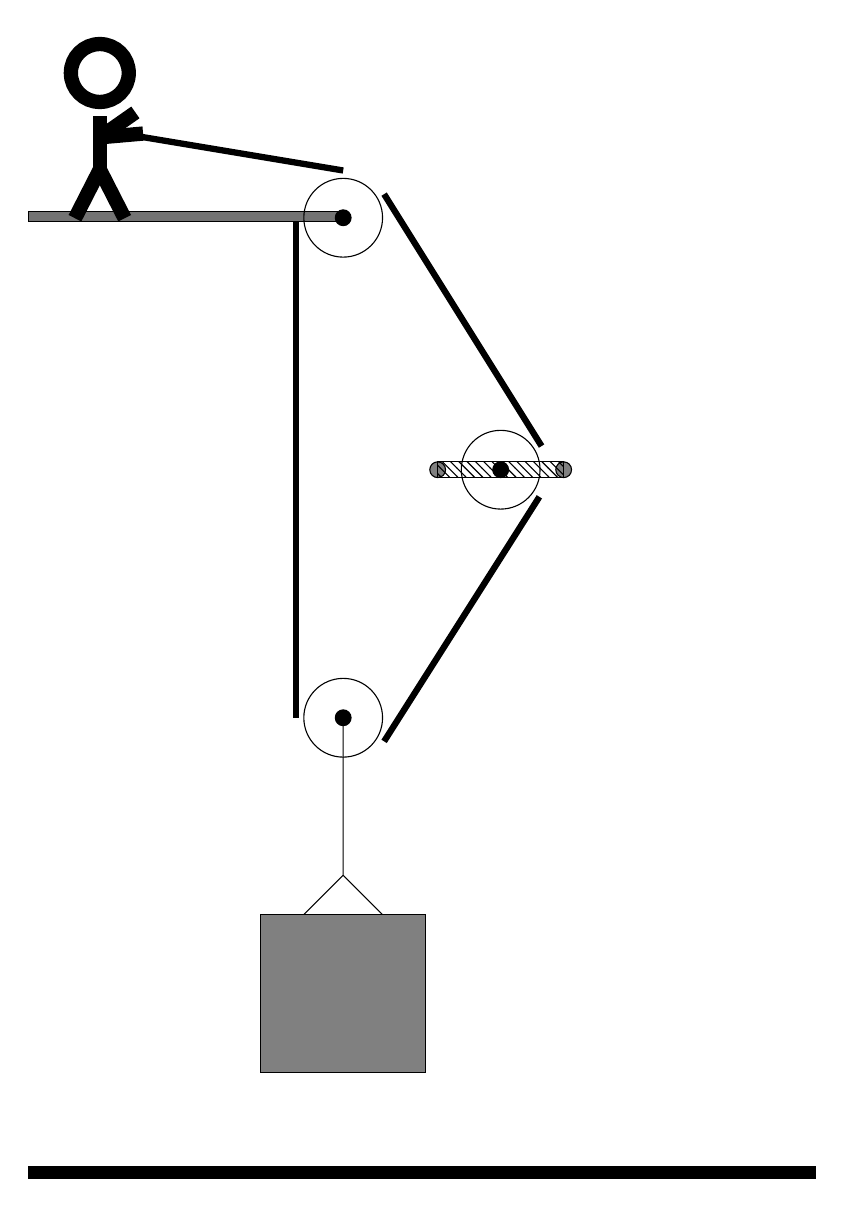
\begin{tikzpicture}
			%%%%% START %%%%%
			\draw[fill=black!55] (-2, 9) rectangle (2, 9.125);
			
			\draw (2, 2.7) circle (0.5);
			\draw[fill=black] (2, 2.7) circle (0.1);
			
			\draw (2, 9.05) circle (0.5);
			\draw[fill=black] (2, 9.05) circle (0.1);
			
			\draw[fill=white](4, 5.85) circle (0.5);
			\draw[fill=black] (4, 5.85) circle (0.1);
			\draw[fill=black!50] (3.2, 5.85) circle (0.1);
			\draw[fill=black!50] (4.8, 5.85) circle (0.1);
			\draw[pattern=north west lines, pattern color=black] (3.2, 5.95) rectangle (4.8, 5.75);
			
			\draw (2, 2.7) -- (2, 0.7) -- (1.5, 0.2) -- (2.5, 0.2) -- (2, 0.7);
			\draw[fill=black!50] (0.95, 0.2) rectangle (3.05, -1.8);
			
			\draw[line width=0.8mm] (1.4, 9) -- (1.4, 2.7);
			\centerarc[line width=0.8mm](2, 2.7)(180:330:0.6);
			\draw[line width=0.8mm](2.5196, 2.4) -- (4.4915, 5.5058);
			\centerarc[line width=0.8mm](4, 5.85)(390:325:0.6);
			\draw[line width=0.8mm](4.5196, 6.15) -- (2.5196, 9.35);
			\centerarc[line width=0.8mm](2, 9.05)(30:90:0.6);
			\draw[line width=0.8mm](2, 9.65) -- (-1, 10.15);
			
			\node at (-1, 10.15) {\Strichmaxerl[10][-175][35]};
			
			\draw[fill=black] (-2, -3) rectangle (8, -3.15);
			%%%%% END %%%%%
		\end{tikzpicture}
	\end{figure}	
\end{document}